\def\stmt{$A$}
% \def\stmt{$\phi$}

% The ability articulate a \emph{degree of confidence} is an important aspect of knowledge representation.
The ability to articulate a \emph{degree of confidence} 
% (or the opposite: a degree of uncertainty)
is a critical aspect of representing knowledge.
% is an important aspect of representing knowledge.
	% Subpoint: it helps avoid a brittleness of always beliving things
	% Subpoint: Protects against overconfidence.
There are 
% Correspondingly, there are
many well-established ways to quantify (un)certinaty \parencite[\S2]{halpern2017reasoning},
	% probability chief among them.	
	and chief among them is probability.
	% perhaps most common is to use probabilities.
% Indeed, many people use ``confidence'' as a synonym for probability.
% Indeed, ``confidence'' is often used as a synonym for probability. 
% Indeed, ``high confidence'' and ``high probability'' are often used interchangably. 
% Indeed, ``confidence'' and 
% In our view, this practice
% Although this use of the word is perfectly functional, it seems to have shadowed another conception of confidence---one that is fundementally different, if at first sublty so.
% However, this practice shadows
% However, this practice seems to have shadowed 
% However, there is also another conception
% However, there
% However, there is also another conception 
% 	of confidence---one that is fundementally different, if at first subtly so.
% Although there is nothing wrong with this, 
% which seems have been shadowed by the enormous success of probability---one that is fundementally different, if at first subtly so.
% which seems to have been shadowed by the enormous success of probability---a concept that is fundementally different, if at first subtly so.
% This paper develops that notion 
% However, there is also another conception of confidence---one that complements traditional representations of uncertainty, and is fundementally different in nature. 
% In our view, however, there is also another conception of confidence:
% 	% one that complements traditional representations of uncertainty, and is fundementally different in nature. 
% 	one that complements traditional representations of uncertainty (such as probability), and is fundementally different in nature. 
% In our view, however, there is also another conception of confidence
This paper, describes a very different conception of confidence
that arises when updating beliefs. 
	% one that complements traditional representations of uncertainty, and is fundementally different in nature. 
% This alternate conception of confidence, which is the focus of the present paper,
% This alternate conception
As we shall see, this notion of confidence
% can be used alongside 
complements traditional representations of uncertainty (such as probability), 
% but is fundementally different in nature. 
and moreover unifies a number of different concepts across computer science.
% ranging from traditional notions of confidence like inverse variance, and Shafer's weight of evidence, to notions in ML and optimization: learning rates and objective strengths. 
% We develop this notion 


% For us, confidence is a measure of trust (in incoming information), rather than of likelihood (of hypothetical information). 
For us, confidence (in an input $\phi$) is a measure of trust, rather than of likelihood;
it quantifies seriously we take $\phi$ in updating our beliefs.
% in an updating context: it's how seriously you take an input
% What we have in mind applies in an updating or learning setting. 
% We take confidence (in an input $\phi$) to be a measure of how seriously we take $\phi$ in updating our beliefs.
% Like probability, confidence lies in continuum between two extremes, but it ranges from untrusted to trusted, rather than from unlikely to likely.
% More concretely, confidence interpolates between prior beliefs and the beliefs one would obtain by fully incorporating $\phi$, so as to obtain posterior beliefs somewhere in between. 
More concretely, confidence interpolates between prior beliefs and those obtained by fully trusting $\phi$, so as to obtain posterior beliefs somewhere in between. 
% This already suffices to characterize our simplest running example:
To take a simple example,
if our prior belief is a probability measure $p(X)$, then to update on event $A$ with confidence $\chi \in [0,1]$ might be to arrive at the posterior belief $p'(X) = (1-\chi) p(X) + (\chi)\, p(X|A)$. 
% In this case, $\chi$ can be viewed as a ``fraction of incorporation''.
Note that 
an update with no confidence ($\chi{=}0$) ignores new information (since $p' \!=\! p$),
while a
% more customary
full confidence update ($\chi{=}1$) takes it as seriously as possible,
% (since then $p'(A) \!=\! 1$).  
since afterwards $p'(A) \!=\! 1$ and there is no way to further incorporate $A$.
% However, there more to it than linear interpolation.
%
In this context, 
full confidence updates are customary, and
the confidence $\chi \in [0,1]$ has a clear interpretation as the ``fraction of the way towards fully incorporating $\phi$''.
% In other cases, however, 
% This is not always true.
In others, however, it may not be clear what 
 	such a number (say, $\chi=0.7$) means.
% In other cases, there are other more natural ways to articulate one's confidence.
% there are other, more natural ways to measure confidence.

% The confidence domain $[0,1]$ 
% In general, it is not clear what a confidence $\chi \in [0,1]$ means, and the scale starts to be less useful.
% In other cases, however, it is not so clear what it means to go, say, ``70\% of the way'' to fully incorparting information. 
% We still have a sensible notion of confidence in these cases, . 
% We now describe such an example.
% One such example is training a neural network. 
Consider a neural network, whose ``belief'' state is a setting of weights,
	which are updated when given a training point.
% As it sees each training point, it updates its weights. 
Modern learning algorithms do not take any individual point too seriously;
% the training data could be full of inconsistencies. 
% For example, 
each training point $x$ changes the weights incrementally, and alone may not even be enough for the network to classify that point correctly.
Thus, there is a significant difference betwen cycling through the training data once, and doing so many times.
Nevertheless, the weights do eventually converge if we repeatedly train on $x$, which is a natural notion of ``fully incorporating $x$''.
% In this context, 
Again we have two extremes: if we have no trust in $x$, we should throw it out; if we trust it completely, we should train until convergence (i.e., the limiting weights after an infinite number of iterations). 
% Now, the number of training iterations is a more 
What does it mean to train the network ``70\% of the way''?
Clearly it doesn't make sense to measure as a fraction of the infinite time taken to get there, and while we could could measure by fraction total distance traveled, it is not clear it is possible to identify such a point without having already trained the network (nearly) to convergence. 
% It doesn't make sense to measure fraction of the total training time, since 
% Rather, in this context, the number of training iterations and the 
In this case, the number of training iterations is a much more convenient measure of confidence. 
% Instead there is a natural scale /$\beta \in [0,\infty]$ that works in all cases.


\begin{figure}
\centering
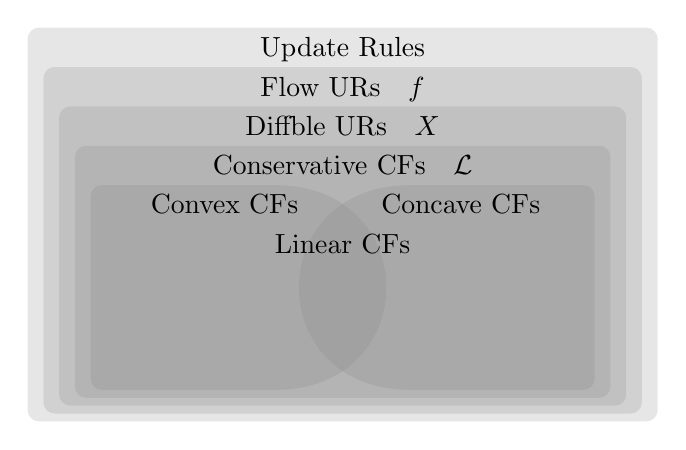
\begin{tikzpicture}
	\begin{scope}[fill=gray,fill opacity=0.2,rounded corners=4px]
		\fill (0,0) rectangle (8,5); % URs (Full Updates)
		\fill[] (0.2,0.1) rectangle (7.8,4.5); % Flow URs (Flows)
		\fill[] (0.4,0.2) rectangle (7.6,4.0); % Diffble URs (Vec Field)
		\fill[] (0.6,0.3) rectangle (7.4,3.5); % Conservative URs 
		\fill (0.8,0.4) -- (0.8, 3.0) -- (3, 3.0)
		 	to[out=0,in=0,looseness=2] (3,0.4) --cycle; % CONVEX
		\fill (7.2,0.4) -- (7.2, 3.0) -- (5, 3.0)
		 	to[out=180,in=180,looseness=2] (5,0.4) --cycle; % CONCAVE
	\end{scope}
	\begin{scope}[anchor=north]
		\node at (4.0, 5.0) {Update Rules};
		\node at (4.0, 4.5) {Flow URs~~~$f$};
		\node at (4.0, 4.0) {Diffble URs~~~$X$};
		% \node at (4.0, 3.5) {Conservative CFs~~~$\mathcal L$};
		\node at (4.0, 3.5) {Conservative CFs~~~$\mathcal L$};
		\node at (2.5, 3.0) {Convex CFs};
		\node at (4.0, 2.5) {Linear CFs};
		\node at (5.5, 3.0) {Concave CFs};
	\end{scope}
\end{tikzpicture}
\caption{%
	hi}
\end{figure}


 % natural measure of confidence that works in all cases,
% which 
It turns out that there is a natural way of measuring confidence in all cases of interest, based on differential geometry of belief space. 
Furthermore, in the case where belief states are Dempster-Shafer belief functions, 
and inputs are simple support functions, this measure of confidence is what Shafer calls the ``weight of evidence''.
%% TODO: Shafer


%%%%% PARAGRAPH ON MANY DIFFERENT VIEWPOINTS
% Linear interpolation, however, is just the tip of 
% At the heart of our paper is a hierarchy 

% It is not always most natural for confidence to range between zero and one. 
% But there are many instances in which 
% However, there is a more universal representation of it in $[0, \infty]$


% Our notion of confidence applies only new information.
Our notion of confidence 
% 	applies to incoming information, rather than to  a belief state
and it is a measure of trust, rather than likelihood.
Like probability, it is a scale between two extremes.
% While probability ranges from untenable (0) to undeniable (1),
% confidence ranges from completely untrustworthy $(\bot)$ to fully trusted ($\top$).
%
% % We apply this notion confidence of updating.
% % This paper explores how confidence works in state-updating context.
% This paper explores how confidence works in the context of learning.
% In this setting, one has some belief state, and recieves inputs, which one might have some degree of confidence in, which is used to modify one's belief state.
% Our use of confidence can be viewed as a measure of how seriously to take an input in updating our beliefs.

High confidence is in many ways like high probability: if we really trust a statement \stmt, we should fully incorporate it into our beliefs, and thereby come to believe it with high probability.
Similarly, it only makes sense to be extremely confident in a \stmt\ if you believe that \stmt\ is extremely likely to be true.
Low confidence, on the other hand, is quite different from low probability.
If we have little trust in \stmt, we should \emph{ignore} \stmt, rather than coming to believe that \stmt\ is unlikely.
% To say \stmt\ has low probabilty is  high confidence in the $\lnot$\stmt.
For example, if an adversary tells you something that you happen to already believe,
% is likely to be true
you might say you have low confidence in their statement, but nevertheless ascribe it high probability.

% The approach we take in this paper is very general,
% Our approach is quite general, and applies any time a belief state is modified in resonse to an input.
% one wants to measure (gradual) incorporation of new information into one's beliefs, and may be thought of as a measure of how much of the new information makes it into one's beliefs.

\subsection{Other Conceptions of Confidence.}

\textbf{Probability.}
% Probability is a numerical scale that ranges from untenable (0) to undeniable (1).
% No number on this scale is truly neutral.
% One of the biggest shortcomings of probability is its inability to represent a truly neutral attitude towards a proposition.
Some people do use ``confidence'' to mean the same thing as probability. When they say they have low confidence in $\phi$, they mean that they think $\phi$ is unlikely.

One of the biggest shortcomings of probability is its inability to represent a truly neutral attitude towards a proposition.
%  probability of $\frac12$ .
% This shortcoming has perhaps been the primary selling point of many alternatives to probabiltiy, such as Dempster-Shafer Belief functions.
A value of $\frac12$ may be equally far from zero as it is from one, but is by no means a neutral assessment in all cases: hearing that your favored candidate has a 50\% chance of winning is big news if a win was previously thought to be inevitable.
For this reason, telling someone the odds are 50/50 is quite different from saying you have no idea.
% By contrast, zero confidence represents a truly neutral stance; a statement with zero confidence has no effect.
By contrast, zero confidence represents something truly neutral:
	a statement made with zero confidence does not stake out a claim, and
	a statement recieved with zero confidence does not affect the recipient's beliefs.
Nevertheless, in some contexts, we will see that confidences correspond to to probabilities.

\textit{Opacity.} To use a graphical metaphor, think of certainty as black or white.
Probability describes shades of gray, while confidence describes opacity.
If we are painting with black and start with a white canvas, there is a precise correspondence between the opacity and the resulting shade of gray.

\textbf{Upper and Lower Probabilities.}
Upper and lower probabilities can describe a neutral attitude towards a proposition, but they are not really a specification of trust, but rather a direct specification of a belief state.
It isn't immediately clear how to use these representations of uncertainty to update, and they're a little too complex to function effectively as the primitive measure of trust that we're after.


\textbf{Shafer's Weight of Evidence.}
Shafer's ``weight of evidence'' is precisely the same concept we have in mind.
Our analysis precsely reduces to his, in the setting where belief states are Belief functions (which generalize probabilities, but not, say, neural network weights), and observations are events.
% This paper can be a generalization of Shafer's ``weight of evidence'' to a broader class of settings, where one might have very different belief states and observations.
Thus, this paper can be viewed as generalizing this concept to a broader class of settings, without requiring that one adopt Shafer's conception of a belief state or an observation.


\textbf{Variance and Entropy.}
The inverse of variance, sometimes known as precision,
	is also commonly used to measure confidence.
If a sensor is unreliable and can give a range of answers, the variance of the estimate is a very common way of quantifying this reliablility.
If measurements have zero variance, in some sense one has absolute confidence ($\top$) in the sensor. If measurements have infinite variance, then in some sense one has no confidence in the sensor, since individual samples convey no information about the true value of the quantity measured.
As with probability, inverse variance will coincide with confidence in some settings; we will see how in \cref{sec:variance}.

Entropy, like variance, is a standard way of measuring uncertainty, and in some settings, confidence coincides with entropy (see \cref{sec:entropy}).
The assumption underlying both approaches is that there's some ``true'' value of the variable, and that the randomness is epsistemic (due to sensor errors) rather than aleotoric (inherrent in the quantity being measured).

\textbf{Confidence Intervals and Error Bars.}
Another notion of the word ``confidence'' comes from the term ``confidence interval''.
This concept arises in settings involving a probability distribution $\Pr(X)$ over a metric space $X$, typically $X = \mathbb R$.
A 95\% confidence interval is the (largest) ball containing 95\% of the probability, and its size is a geometric measurement of how .
This intuition behind this reading of the word confidence is the same as
